\documentclass[12pt,letterpaper]{article}


\newcommand{\studentname}{Ben Bassett}
\newcommand{\labpartner}{Katrina Sumarli}

\title{\textsc{Lab 02: Harmonic Oscillator with Air Drag}}
\newcommand{\shorttitle}{Harmonic Oscillator with Drag}

\newcommand{\course}{PHY310}
\newcommand{\labdate}{09-10-2024}

%------------------------------------------------------------------------------------------------------------

\usepackage[letterpaper,left=1in,right=1in,bottom=1in,top=1in]{geometry}
\usepackage{fancyhdr}
\usepackage{subfigure}
\usepackage{graphicx}
\usepackage{amsmath}
\usepackage{cleveref}
\usepackage{booktabs}
\usepackage[british]{babel}
\usepackage[square,comma,numbers,sort&compress]{natbib}
\usepackage{csvsimple}
\usepackage{graphicx}
\usepackage{pgfplotstable}
\usepackage{textcomp,gensymb}
\usepackage{array}
\usepackage{tabu}
\usepackage{multirow}
\usepackage{url}
\usepackage{lipsum}
\pgfplotsset{compat=1.9}% supress warning
\begin{document}

%------------------------------------------------------------------------------------------------------------

\setlength{\parindent}{1em}
\setlength{\parskip}{0.5em}
\author{\course~Lab Journal \\ \\ \studentname\,\& \labpartner}
\date{\labdate}

\renewcommand\abstractname{Summary}

\pagestyle{fancy}
\fancyhead{}
\fancyhead[l]{\course:~\shorttitle}
\fancyhead[r]{\studentname}
\fancyfoot{}
\fancyfoot[C]{\thepage}
\renewcommand{\headrulewidth}{0pt}
\renewcommand{\footrulewidth}{0pt}

\renewcommand\bibname{References}

%------------------------------------------------------------------------------------------------------------

\renewcommand\abstractname{Abstract}
\maketitle

% COMMENT IN IF ASKED TO SUBMIT REPORT WITH ABSTRACT
%\begin{abstract}
%Maximum 200 words.
%\end{abstract}

\section{Purpose}
This lab aimed to measure the coefficient of air drag as a function of cross-sectional area.

\section{Experimental Apparatus}

\lipsum[1]

Our general setup is illustrated in Figure \ref{fig:setup}.

 \begin{figure}[h]
     \centering
     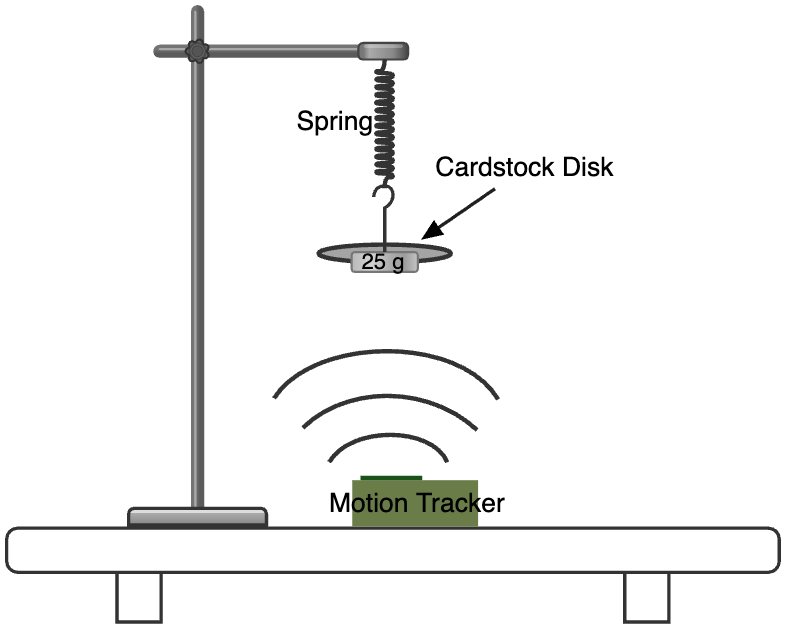
\includegraphics[width=4in]{images/setup.png}
     \caption{A diagram of our experimental setup}
     \label{fig:setup}
 \end{figure}

\pagebreak
\section{Procedure}

\lipsum[1]

\section{Results}

\lipsum[1]

\begin{equation}
    F_D=3\pi \mu Dv
\end{equation}

 \begin{figure}[h]
     \centering
     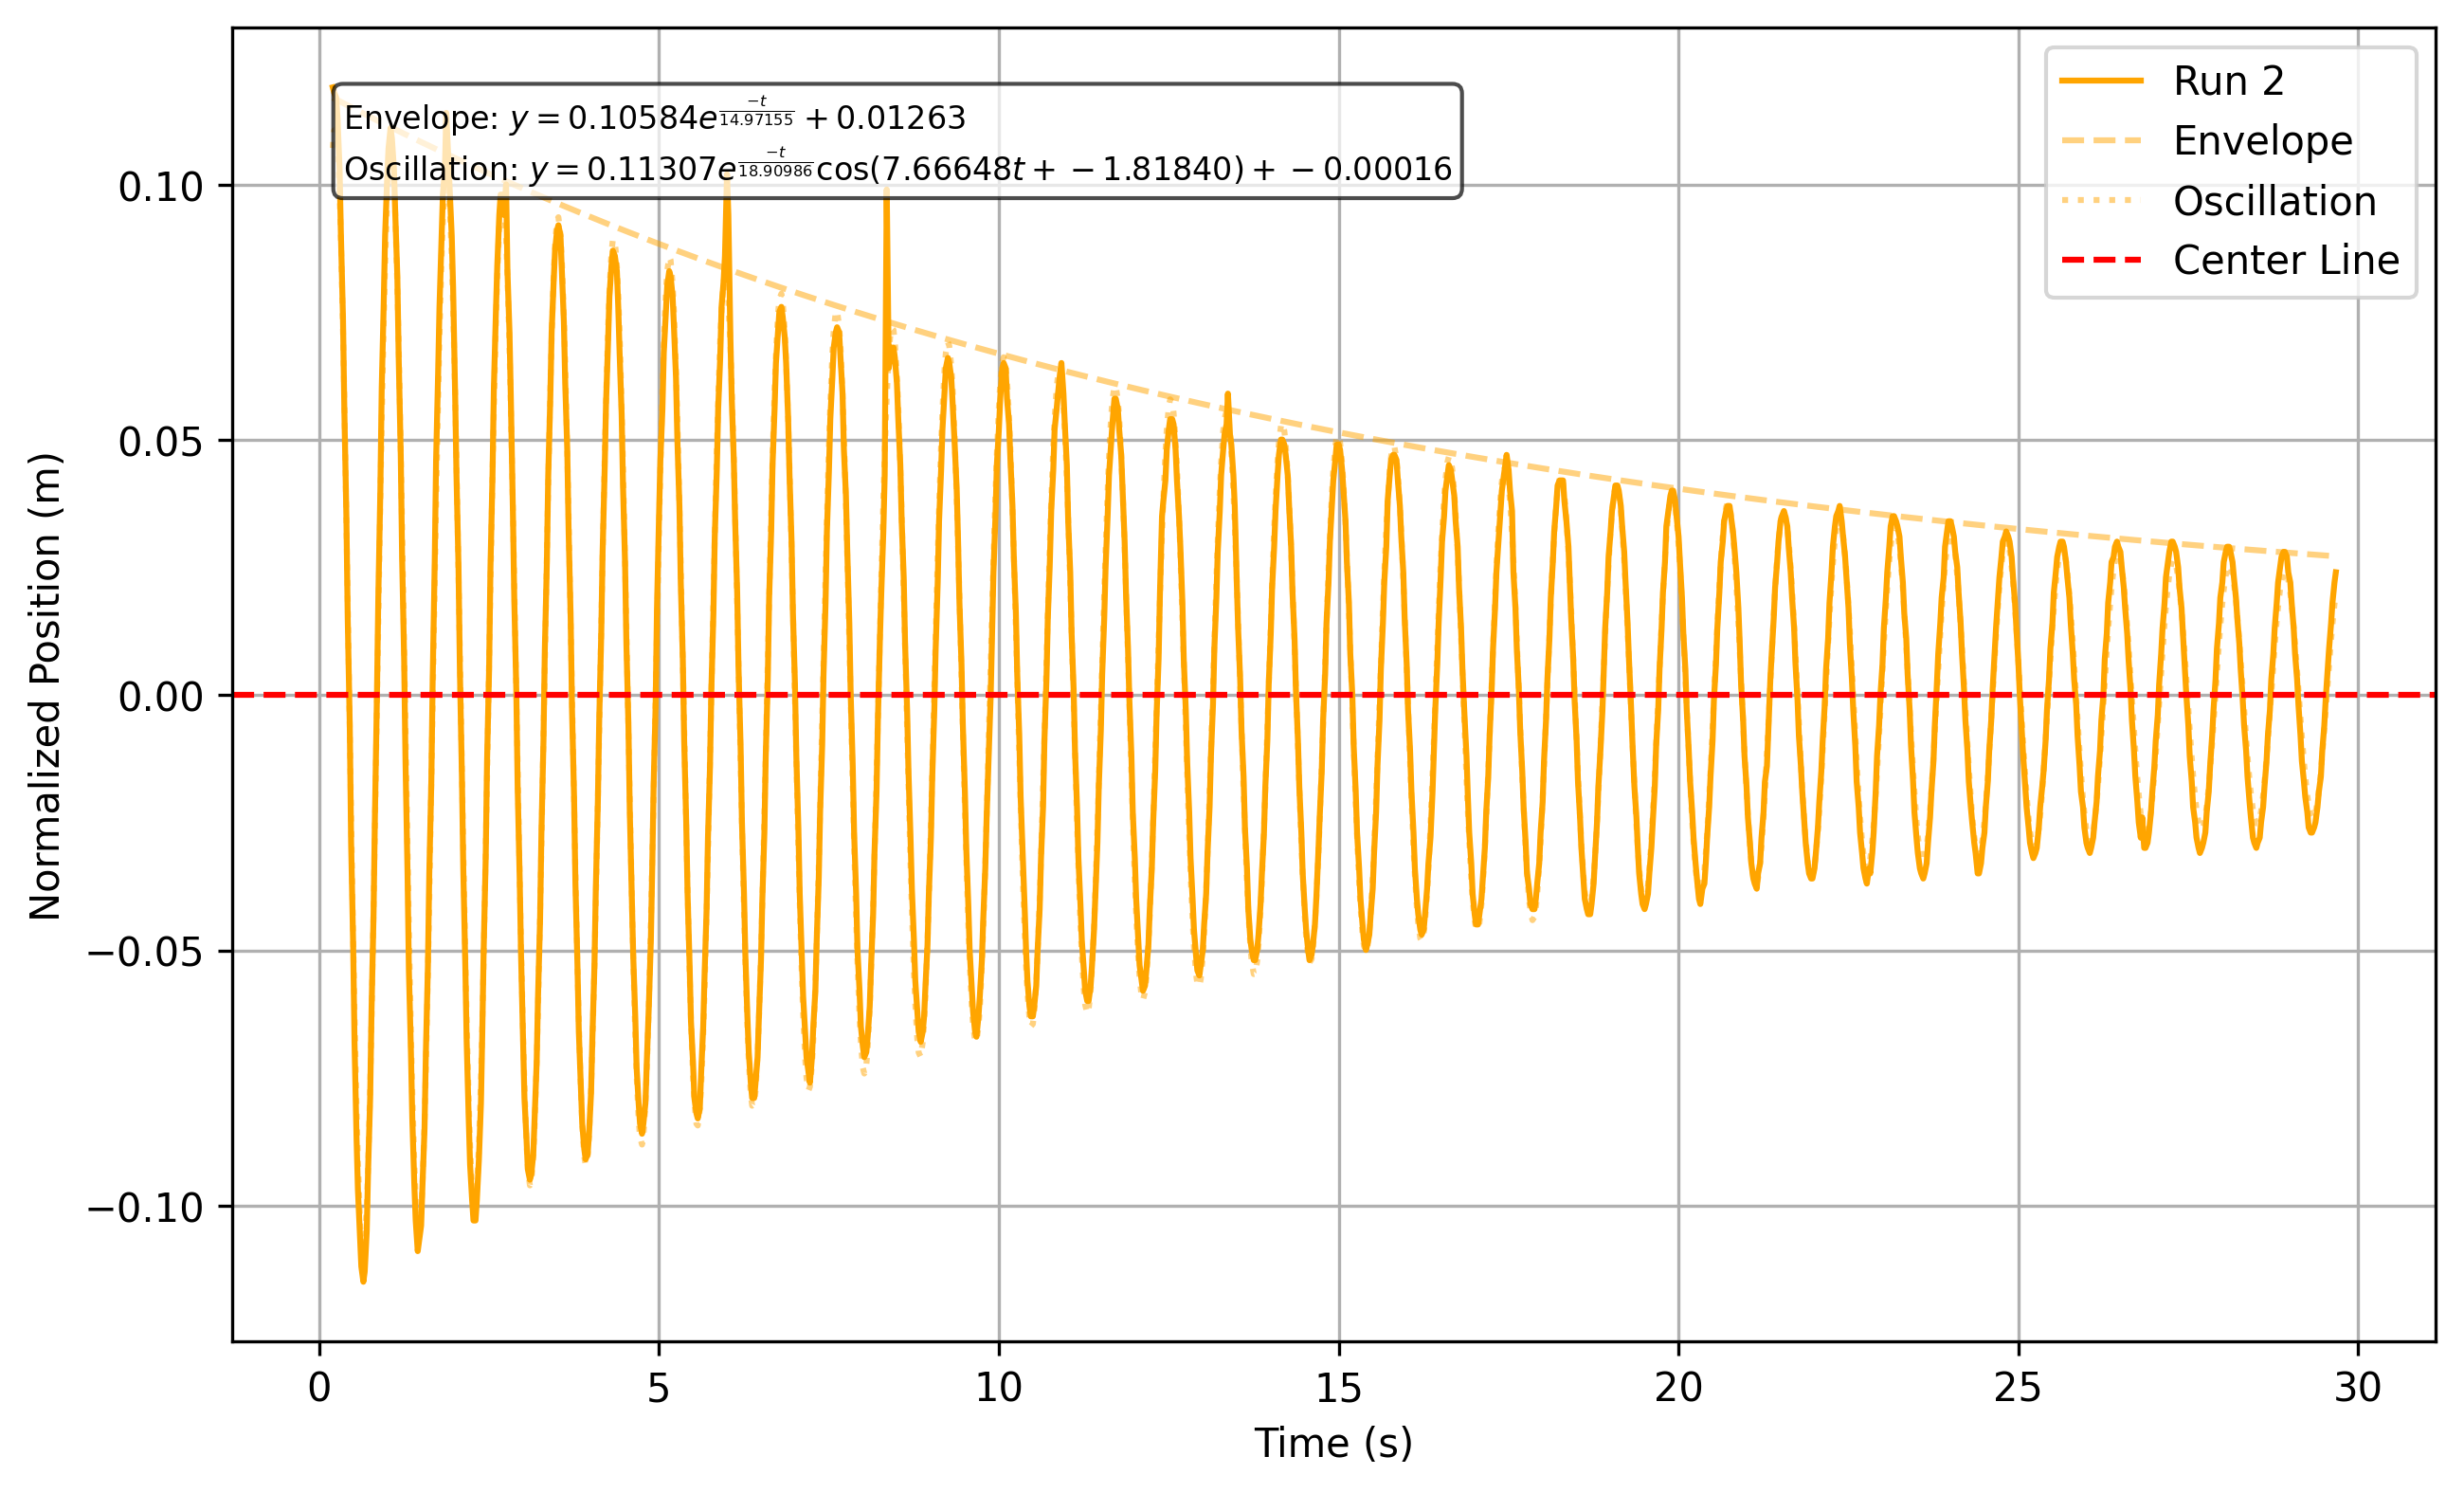
\includegraphics[width=4in]{images/4cm.png}
     \caption{The spring with a 4 cm disc}
     \label{fig:4cm}
 \end{figure}

  \begin{figure}[h]
     \centering
     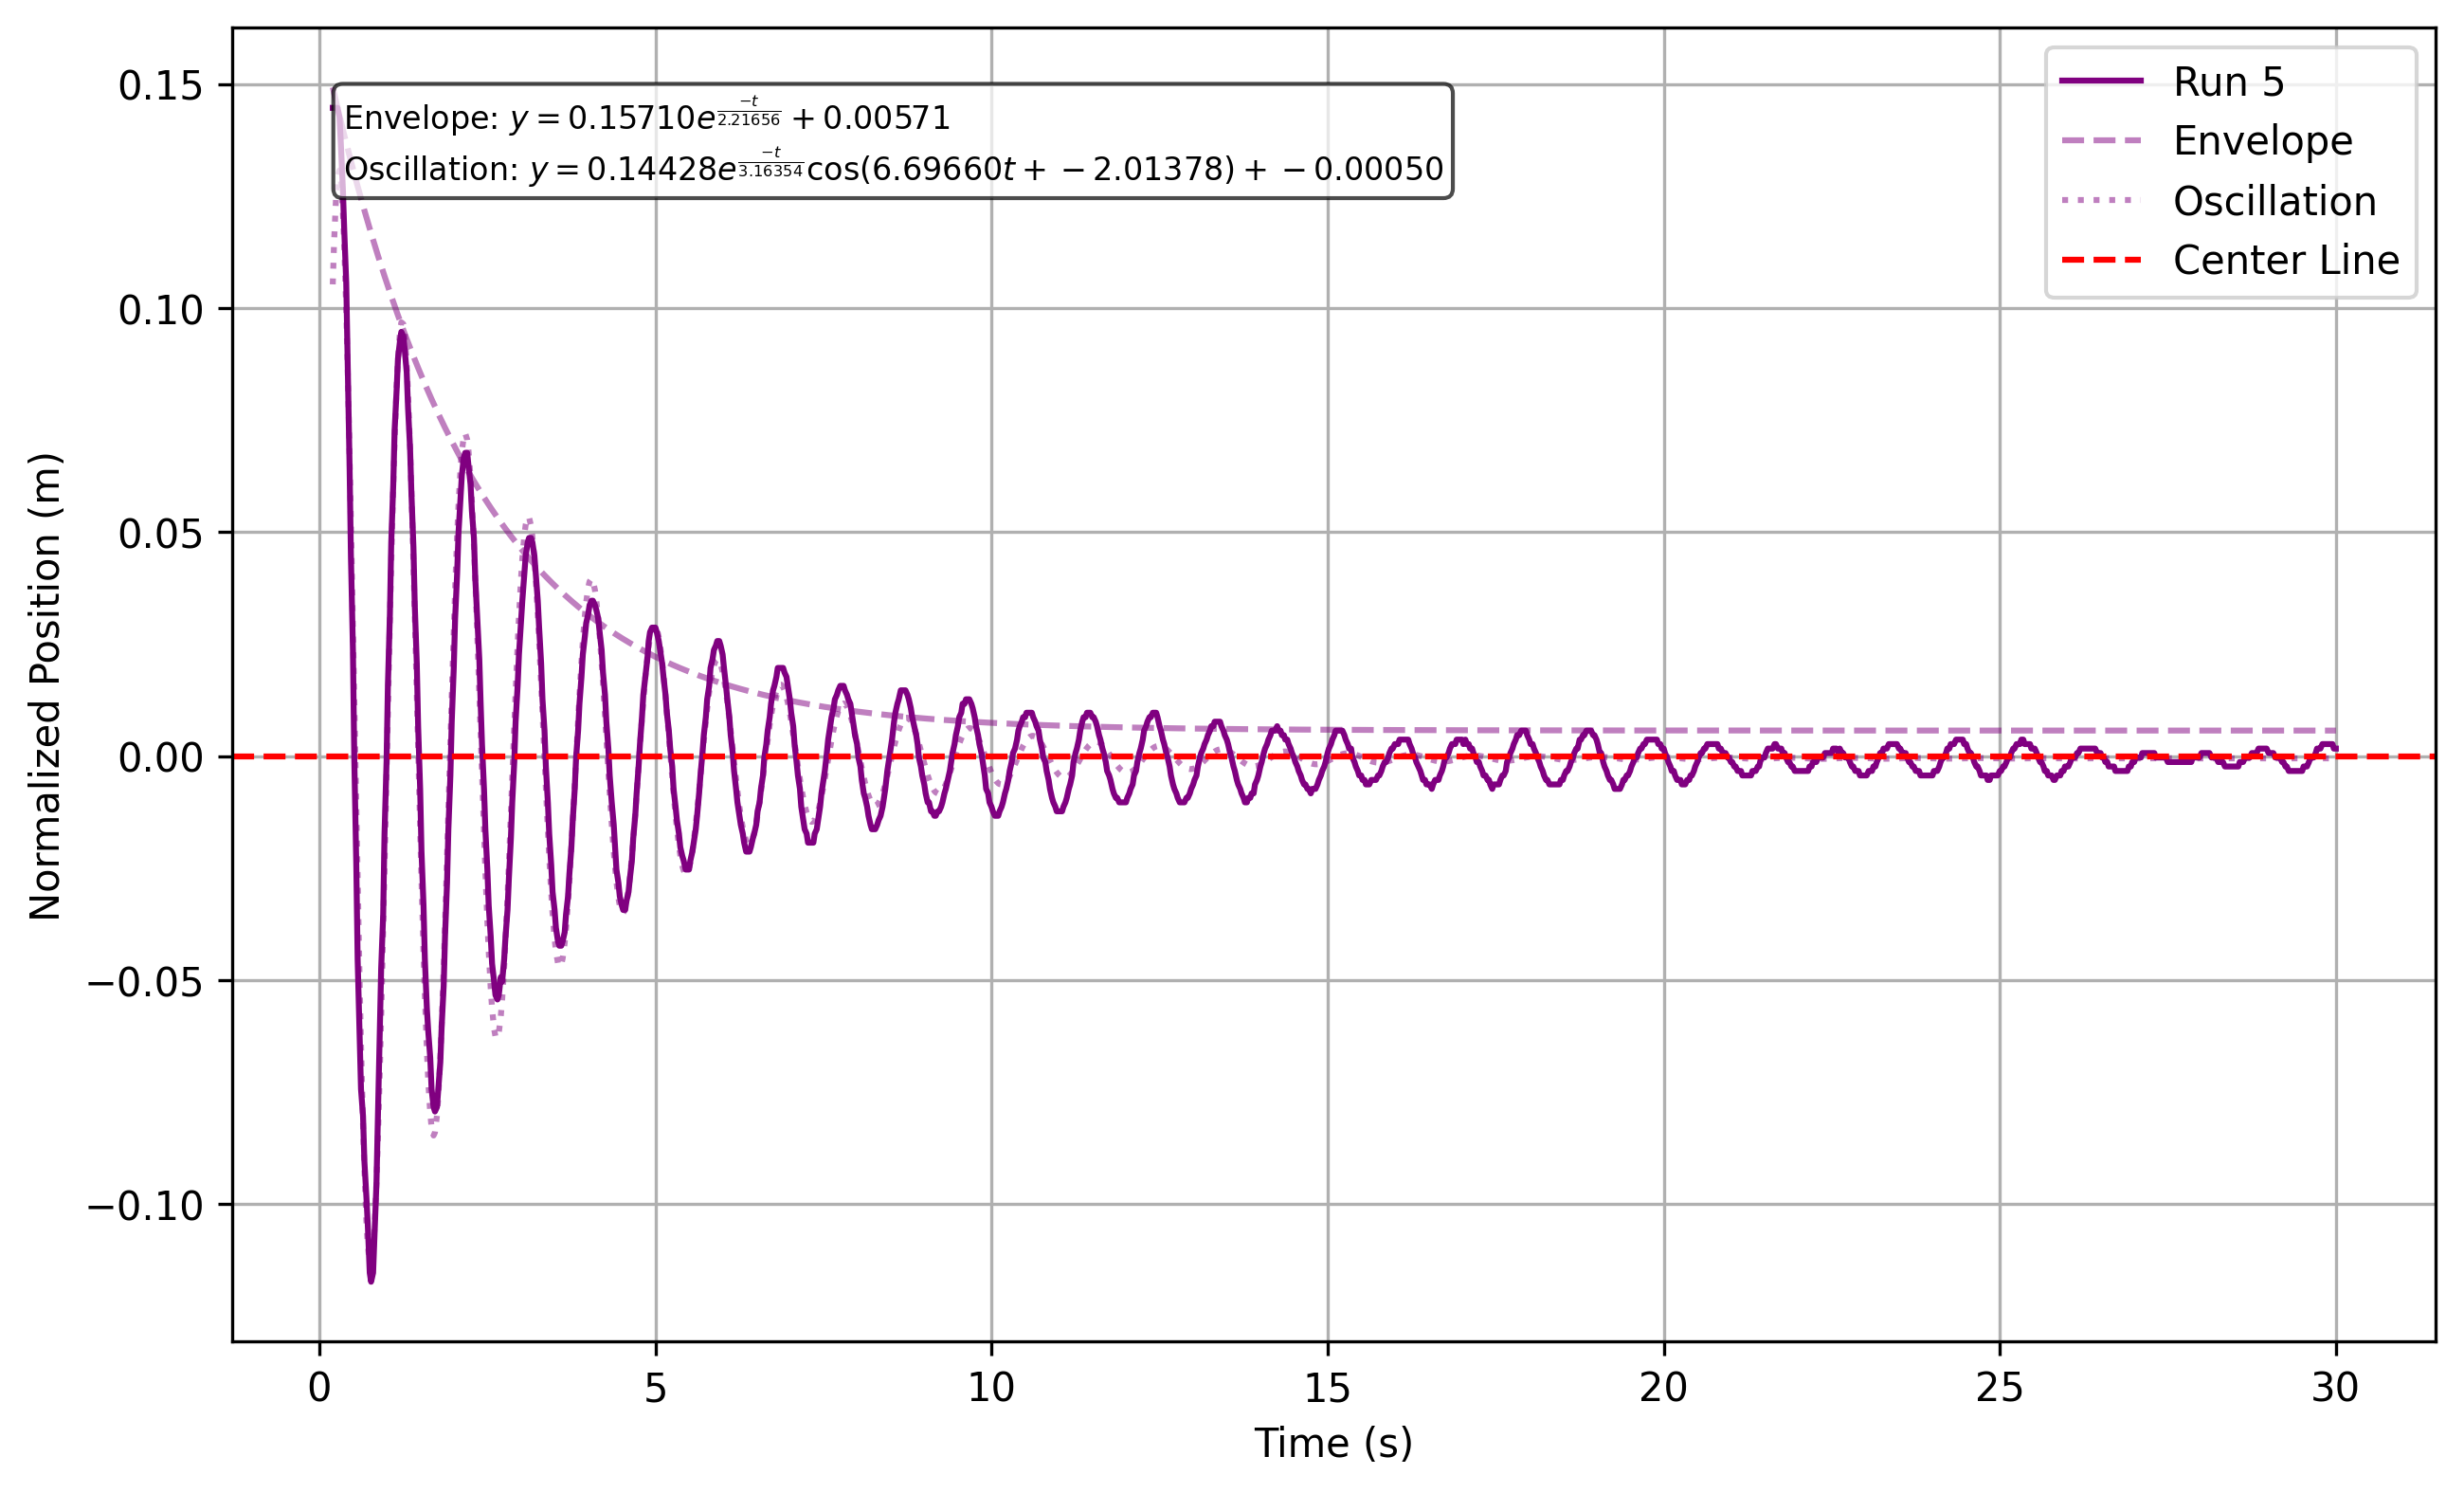
\includegraphics[width=4in]{images/10cm.png}
     \caption{The spring with a 10 cm disc}
     \label{fig:10cm}
 \end{figure}

\section{Conclusions}

\lipsum[1]


% \bibliographystyle{unsrtnat}
% \bibliography{references}

\end{document}
